% ======================================================================
% CAPÍTULO 3: DATASET FATIGUESET Y PROCESAMIENTO DE SEÑALES FISIOLÓGICAS (EXPANDIDO)
% ======================================================================

\chapter{Dataset FatigueSet y Procesamiento de Señales Fisiológicas}
\label{cap:dataset_preprocesamiento}

\section{El Benchmark Multimodal FatigueSet}
\label{sec:fatigueset_benchmark}

El conjunto de datos \fatigueset{} \cite{kalanadhabhatta2021fatigueset, kalanadhabhatta2022fatigueset} representa un hito fundamental en el campo de la computación vestible (\textit{wearable computing}), el procesamiento de bioseñales y la monitorización de la salud digital. A diferencia de conjuntos de datos biomédicos tradicionales confinados a entornos clínicos controlados con instrumentación fija y voluminosa de grado médico, \fatigueset{} recopila de manera continua y sincronizada bioseñales multimodales mediante cuatro dispositivos comerciales no invasivos a lo largo de protocolos estandarizados de inducción de fatiga física y mental en condiciones semi-controladas.

\subsection{Cohorte de Participantes y Diseño Experimental}

La cohorte experimental estuvo compuesta por 12 participantes adultos jóvenes sanos ($N=12$, identificados de P01 a P12), con edades comprendidas entre los 20 y 32 años, con representatividad balanceada en cuanto a hábitos de actividad física. Cada sujeto completó tres sesiones de experimentación independientes en días distintos para cada modalidad de fatiga (física y cognitiva), estructuradas bajo un diseño de bloques contrapesados (\textit{counterbalanced block design}) para neutralizar el efecto de orden, habituación y aprendizaje motor. La estructura protocolar completa de cada sesión se detalla esquemáticamente en la Figura~\ref{fig:protocolo_sesion_detallado}.

\begin{figure}[htbp]
    \centering
    \resizebox{\linewidth}{!}{%
    \begin{tikzpicture}[node distance=0.8cm, auto,
        survey/.style={ellipse, draw=ugrred, fill=red!6, text width=2.4cm, text centered, minimum height=1.1cm, font=\scriptsize},
        task/.style={rectangle, draw=etsiitblue, fill=blue!6, rounded corners, text width=3.2cm, text centered, minimum height=1.4cm, font=\scriptsize},
        line/.style={draw=darkblue, -latex', thick}]
        
        \node [survey] (baseline) {\textbf{Evaluación Basal}\\SSS, GVAS, FSS};
        \node [task, right=0.5cm of baseline] (block1) {\textbf{Bloque 1 (30 min)}\\Tarea Cognitiva/Física\\(Intensidad Baja)};
        \node [survey, right=0.5cm of block1] (eval1) {\textbf{Auto-reporte}\\VAS (Fís/Men)};
        \node [task, right=0.5cm of eval1] (block2) {\textbf{Bloque 2 (30 min)}\\Tarea Cognitiva/Física\\(Intensidad Media/Alta)};
        \node [survey, right=0.5cm of block2] (eval2) {\textbf{Evaluación Final}\\Post-Task Survey};
        
        \path [line] (baseline) -- (block1);
        \path [line] (block1) -- (eval1);
        \path [line] (eval1) -- (block2);
        \path [line] (block2) -- (eval2);
    \end{tikzpicture}%
    }
    \caption{Estructura protocolar de una sesión experimental en \fatigueset{} con evaluaciones basales, bloques de inducción graduada y auto-reportes continuos VAS.}
    \label{fig:protocolo_sesion_detallado}
\end{figure}

El protocolo experimental sometió a los participantes a dos categorías estructuradas de inducción de fatiga:
\begin{enumerate}
    \item \textbf{Protocolo de Fatiga Cognitiva (Mental):}
    \begin{itemize}
        \item \textit{Tarea N-Back (Memoria de Trabajo y Atención Sostenida):} Presentación secuencial de letras cada 2 segundos. El participante presiona un actuador si la letra actual coincide con la mostrada $N$ pasos atrás ($N=1$ para intensidad baja, $N=2$ para media y $N=3$ para alta).
        \item \textit{Test de Interferencia de Stroop (Control Inhibitorio y Flexibilidad):} Presentación rápida de palabras de colores con congruencia o incongruencia cromática (p.~ej., la palabra "AZUL" en tinta roja), exigiendo inhibir la lectura semántica y seleccionar el color del texto.
        \item \textit{Aritmética Mental Acelerada:} Series de restas sucesivas de 7 o 13 desde números aleatorios de cuatro dígitos bajo restricciones de tiempo decrecientes.
    \end{itemize}
    \item \textbf{Protocolo de Fatiga Física (Cardiovascular y Muscular):}
    \begin{itemize}
        \item \textit{Cinta Rodante Ergonométrica:} Marcha a 4 km/h con pendiente $0\%$ (baja intensidad), trote a 7 km/h con pendiente $2\%$ (media intensidad) y carrera a 10 km/h con pendiente $5\%$ (alta intensidad).
        \item \textit{Cicloergómetro con Control de Carga:} Pedaleo continuo con potencia controlada fijada en 50 W (baja), 100 W (media) y 150 W (alta intensidad).
    \end{itemize}
\end{enumerate}

\subsection{Cuestionarios Psicométricos y Etiquetas de Regresión Continua}

La evaluación del estado subjetivo del participante se articuló mediante instrumentos psicométricos validados internacionalmente:
\begin{itemize}
    \item \textbf{Escala de Somnolencia de Stanford (SSS):} Escala ordinal de 1 (totalmente alerta y activo) a 7 (luchando contra el sueño) administrada antes de cada sesión \cite{hoddes1973quantification}.
    \item \textbf{Global Vigour and Affect Scale (GVAS):} Evalúa los niveles basales de vigor físico y estado afectivo mediante escalas continuas.
    \item \textbf{Fatigue Severity Scale (FSS):} Cuestionario psicométrico de 9 ítems que evalúa el impacto de la fatiga en el funcionamiento cotidiano.
    \item \textbf{Etiquetas Continuas de Fatiga Física y Mental (VAS 0--100):} Tras cada bloque experimental, los sujetos anotaron su percepción instantánea de fatiga física y fatiga mental sobre una escala visual analógica continua de 100 mm sin marcas intermedias. Estas mediciones normalizadas constituyen el vector objetivo de regresión continua multivariante $\bm{y} \in [0, 100]^2$.
\end{itemize}



\section{Desglose Técnico de los Cuatro Dispositivos Vestibles (23 Canales)}
\label{sec:sensores_tecnicos}

El dataset consolida 23 archivos CSV independientes por sesión, correspondientes a cuatro dispositivos vestibles complementarios, cuyas características físicas y técnicas se detallan en la Tabla~\ref{tab:sensores_canales_fatigueset}.

\begin{table}[htbp]
\centering
\caption{Catálogo técnico de dispositivos, archivos de datos y canales fisiológicos en \fatigueset{}.}
\label{tab:sensores_canales_fatigueset}
\scriptsize
\renewcommand{\arraystretch}{0.88}
\begin{tabularx}{\linewidth}{@{}llXccc@{}}
\toprule
\textbf{Dispositivo} & \textbf{Archivo CSV} & \textbf{Magnitud Física / Canales} & \textbf{$f_s$ Orig.} & \textbf{Rango / Unidad} & \textbf{Tipo} \\
\midrule
\multirow{3}{*}{\textbf{Nokia eSense}} 
& \code{ear\_acc\_left/right} & Aceleración triaxial bilateral ($a_x, a_y, a_z$) & 100 Hz & $\pm 2g$ & Inercial \\
& \code{ear\_gyro\_left/right} & Velocidad angular bilateral ($g_x, g_y, g_z$) & 100 Hz & $\pm 500^\circ/\text{s}$ & Inercial \\
& \code{ear\_ppg\_left/right} & Fotopletismografía óptica (Verde, IR, Rojo) & 100 Hz & Intensidad óptica & Óptico \\
\midrule
\multirow{5}{*}{\textbf{Muse S}} 
& \code{forehead\_eeg\_raw} & EEG 4 electrodos secos (TP9, AF7, AF8, TP10) & 256 Hz & $0 - 1682.8\,\mu\text{V}$ & Electrofisiol. \\
& \code{forehead\_eeg\_[band]} & Potencia absoluta bandas $\delta, \theta, \alpha, \beta, \gamma$ & 10 Hz & Bels & Espectral \\
& \code{forehead\_acc/gyro} & Acelerometría y giroscopio frontal & 52 Hz & $\pm 2g / \pm 245^\circ/\text{s}$ & Inercial \\
& \code{muse\_blinks/clenches} & Detección de parpadeos y tensión mandibular & 10 Hz & Binario $\{0, 1\}$ & Eventos \\
& \code{muse\_device\_fit} & Calidad de contacto piel-electrodo & 10 Hz & Escala $\{1, 2, 4\}$ & Diagnóstico \\
\midrule
\multirow{5}{*}{\textbf{Zephyr 3.0}} 
& \code{chest\_raw\_ecg} & ECG torácico continuo (12 bits) & 250 Hz & $0 - 4095$ bits & Electrocardiog. \\
& \code{chest\_raw\_breathing} & Señal respiratoria mecánica por presión & 25 Hz & 24 bits & Pletismog. \\
& \code{chest\_physiology\_sum} & Resumen continuo: HR, BR, HRV-SDNN & 1 Hz & bpm / rpm / ms & Procesado \\
& \code{chest\_rr/bb\_interval} & Duración de intervalos inter-latido / respiración & Evento & Milisegundos & Eventos \\
& \code{chest\_raw\_acc} & Acelerómetro triaxial torácico & 100 Hz & $\pm 16g$ & Inercial \\
\midrule
\multirow{4}{*}{\textbf{Empatica E4}} 
& \code{wrist\_bvp} & Fotopletismografía de muñeca (BVP) & 64 Hz & Flujo reflectancia & Óptico \\
& \code{wrist\_eda} & Actividad electrodérmica ($\text{Ag/AgCl}$) & 4 Hz & $0.01 - 100\,\mu\text{S}$ & Conductancia \\
& \code{wrist\_skin\_temp} & Temperatura dérmica por infrarrojos & 4 Hz & $0.02^\circ\text{C}$ resol. & Térmico \\
& \code{wrist\_acc} & Acelerometría triaxial de muñeca & 32 Hz & $\pm 2g$ & Inercial \\
\bottomrule
\end{tabularx}
\end{table}



\section{Pipeline Integral de Preprocesamiento y Sincronización Temporal}
\label{sec:preprocesamiento_pipeline}

El procesamiento de flujos biomédicos multimodales heterogéneos impone el diseño de un pipeline riguroso y modular que transforme los 23 flujos de datos crudos en tensores regulares y limpios. La Figura~\ref{fig:pipeline_preprocesado_tikz} ilustra la arquitectura de datos desarrollada en este proyecto.

\begin{figure}[htbp]
    \centering
    \resizebox{\linewidth}{!}{%
    \begin{tikzpicture}[node distance=1.1cm, auto,
        inputblock/.style={rectangle, draw=etsiitblue, fill=blue!8, rounded corners, text width=2.6cm, text centered, minimum height=1.2cm, font=\scriptsize},
        procblock/.style={rectangle, draw=ugrred, fill=red!6, rounded corners, text width=2.8cm, text centered, minimum height=1.2cm, font=\scriptsize},
        outblock/.style={rectangle, draw=darkgreen, fill=green!8, rounded corners, text width=2.8cm, text centered, minimum height=1.2cm, font=\scriptsize},
        line/.style={draw=darkblue, -latex', thick}]
        
        \node [inputblock] (raw) {\textbf{Ingesta Multimodal}\\23 Archivos CSV\\$f_s \in [1, 256]\,\text{Hz}$};
        \node [procblock, right=0.6cm of raw] (resample) {\textbf{Remuestreo Polifásico}\\Filtro FIR Anti-aliasing\\$f_{\text{target}} = 64\,\text{Hz}$};
        \node [procblock, right=0.6cm of resample] (filter) {\textbf{Filtrado Digital}\\Butterworth IIR Fase 0\\Notch 50 Hz por Canal};
        \node [procblock, below=0.8cm of filter] (window) {\textbf{Ventana Deslizante}\\$W=60\,\text{s},\, \Delta=30\,\text{s}$\\$3840 \times C$ muestras};
        \node [procblock, left=0.6cm of window] (features) {\textbf{Extracción Features}\\Temporal, Welch PSD\\SampEn, Poincaré};
        \node [outblock, left=0.6cm of features] (tensors) {\textbf{Tensores PyTorch}\\GroupKFold por Sujeto\\RobustScaler};
        
        \path [line] (raw) -- (resample);
        \path [line] (resample) -- (filter);
        \path [line] (filter) -- (window);
        \path [line] (window) -- (features);
        \path [line] (features) -- (tensors);
    \end{tikzpicture}%
    }
    \caption{Diagrama de bloques del pipeline integral de preprocesamiento, sincronización y estructuración de bioseñales en \code{fatigueset-lib}.}
    \label{fig:pipeline_preprocesado_tikz}
\end{figure}

\clearpage
\subsection{El Problema de la Desalineación Temporal Asíncrona}

En un sistema multimodal real con múltiples dispositivos inalámbricos independientes, cada sensor adquiere datos gobernado por su propio oscilador de cuarzo interno. Como se ilustra en la Figura~\ref{fig:senales_desalineadas_raw}, las bioseñales crudas operan sobre escalas temporales totalmente dispares: la frecuencia cardíaca de Zephyr se registra a $\approx 1\,\text{Hz}$, la actividad electrodérmica de Empatica E4 a $\approx 4\,\text{Hz}$ y los electrodos de Muse S a $\approx 256\,\text{Hz}$. Además de la diferencia de frecuencias, los instantes de muestreo no son coincidentes ($t_i^{\text{chest}} \neq t_j^{\text{wrist}} \neq t_k^{\text{head}}$), impidiendo la construcción directa de una matriz o tensor multivariado unificado.

\begin{figure}[H]
    \centering
    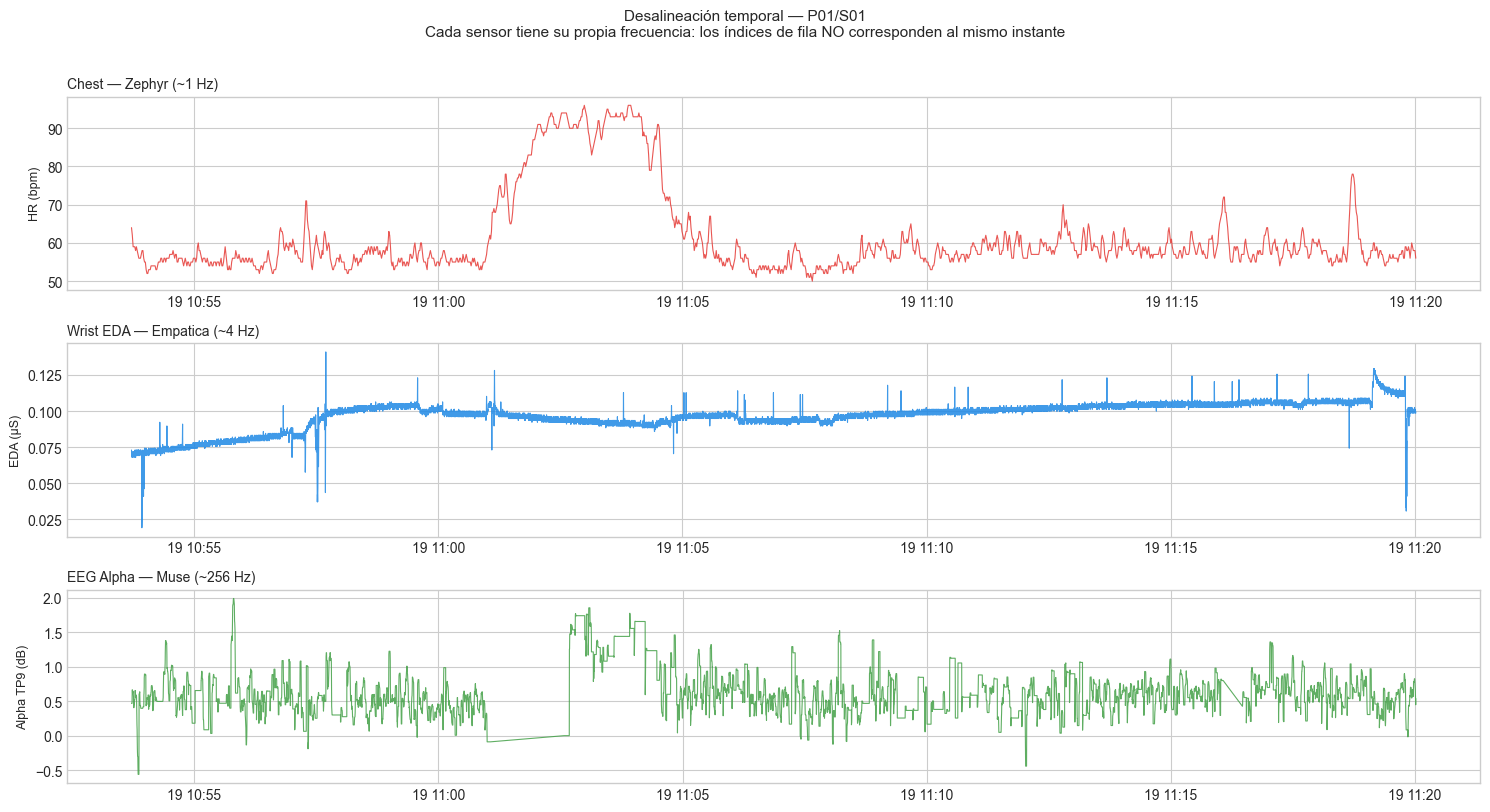
\includegraphics[width=0.84\textwidth]{figures/sincronizacion_senales_desalineadas.png}
    \caption{Señales biomédicas crudas y desalineadas temporalmente de tres dispositivos vestibles en sus propios ejes de tiempo independientes: Zephyr BioHarness ($\sim 1\,\text{Hz}$), Empatica E4 ($\sim 4\,\text{Hz}$) y Muse S ($\sim 256\,\text{Hz}$).}
    \label{fig:senales_desalineadas_raw}
\end{figure}

\subsection{Resampling: Principios de Downsampling y Upsampling}

Para unificar la tasa de muestreo se requiere una combinación de dos operaciones fundamentales:
\begin{enumerate}
    \item \textbf{Diezmado o Submuestreo (\textit{Downsampling}):} Reducción de la frecuencia de muestreo de una señal de alta velocidad (p.~ej., EEG a 256 Hz diezmado a 64 Hz). Si se realizara descartando muestras directamente, se violaría el teorema de Nyquist-Shannon ($f_s \ge 2 f_{\max}$), provocando que las frecuencias por encima de $\frac{f_{\text{target}}}{2} = 32\,\text{Hz}$ se solapen como componentes espurias (\textit{aliasing}). Por ello, es imperativo aplicar previamente un filtro paso-bajo anti-aliasing.
    \item \textbf{Sobremuestreo o Interpolación (\textit{Upsampling}):} Incremento de la tasa de muestreo para señales de baja frecuencia (p.~ej., EDA a 4 Hz elevada a 64 Hz). Consiste en intercalar ceros temporales seguido de un filtro de reconstrucción paso-bajo para suavizar las transiciones.
\end{enumerate}

\subsection{Evaluación de Métodos de Interpolación Temporal}

Para evaluar la reconstrucción de señales tras el sobremuestreo, se contrastaron tres métodos numéricos de interpolación sobre intervalos continuos de 5 minutos, cuyos perfiles se comparan en la Figura~\ref{fig:comparacion_interpolacion}:
\begin{itemize}
    \item \textbf{Vecino más Próximo (\textit{Nearest-Neighbor}):} Asigna a cada instante temporal el valor de la muestra más cercana. Genera discontinuidades en escalera que introducen armónicos espurios de alta frecuencia.
    \item \textbf{Interpolación Lineal:} Conecta puntos adyacentes mediante segmentos rectos. Preserva la continuidad de primer orden pero produce vértices angulosos en los puntos de inflexión.
    \item \textbf{Spline Cúbica (\textit{Cubic Spline}):} Ajusta polinomios cúbicos por tramos garantizando continuidad hasta la segunda derivada ($C^2$). Ofrece una reconstrucción morfológica suave y biológicamente plausible, idónea para bioseñales como EDA o fotopletismografía.
\end{itemize}

\begin{figure}[htbp]
    \centering
    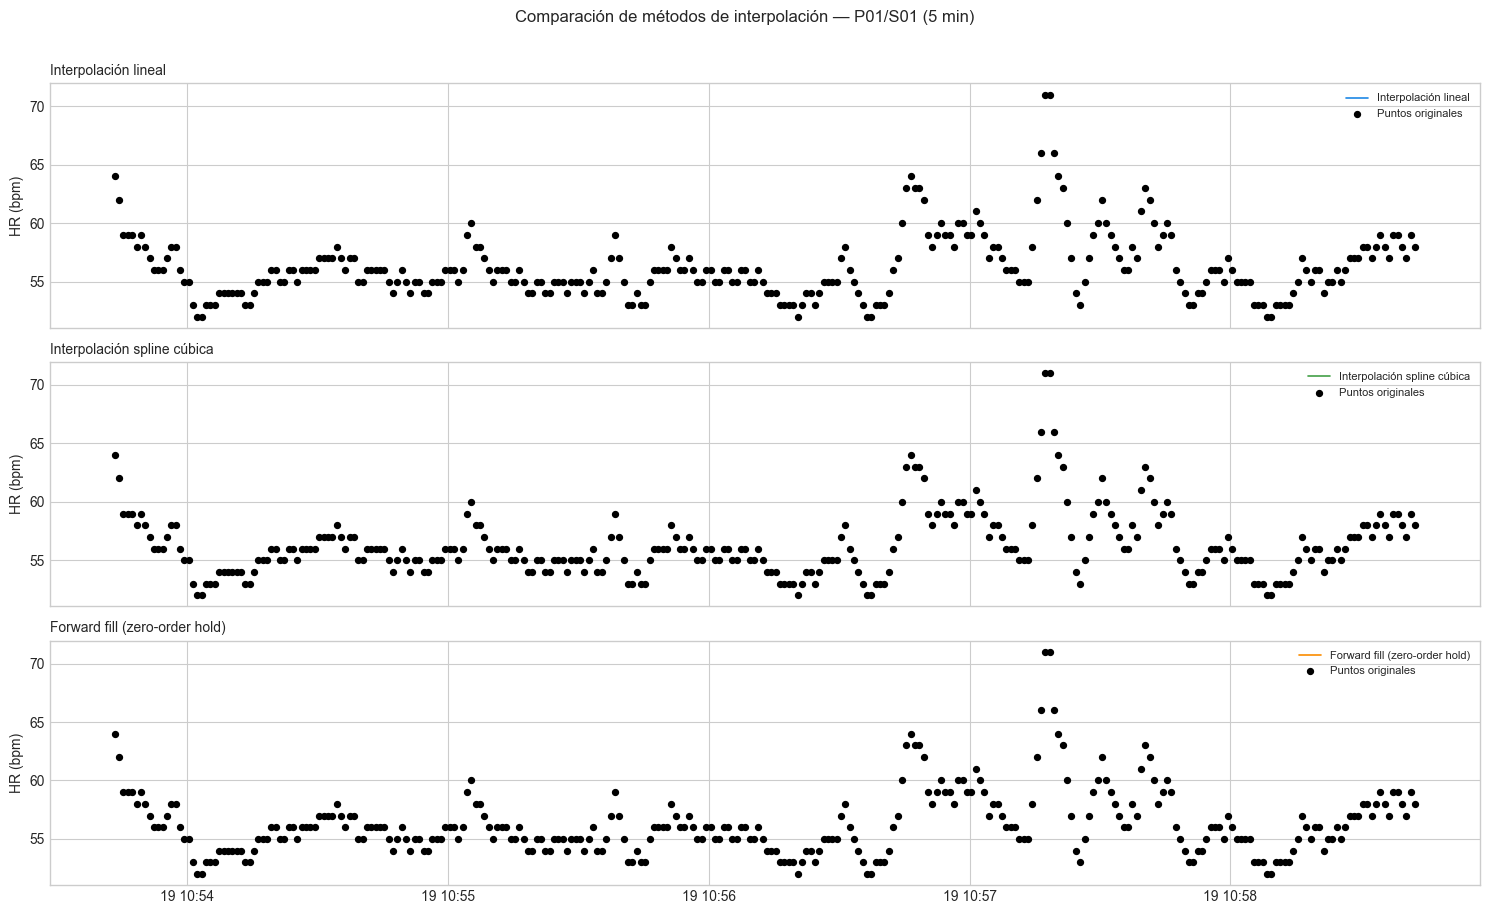
\includegraphics[width=0.88\textwidth]{figures/sincronizacion_metodos_interpolacion.png}
    \caption{Comparación empírica de algoritmos de interpolación temporal sobre una ventana continua de 5 minutos: Vecino más próximo (Nearest), Interpolación Lineal y Spline Cúbica.}
    \label{fig:comparacion_interpolacion}
\end{figure}

\subsection{Pipeline Completo de Sincronización a 64 Hz}

En lugar de interpolaciones desacopladas, en \code{fatigueset-lib} se implementa el remuestreo polifásico con filtrado anti-aliasing mediante \code{scipy.signal.resample\_poly}. Para transformar una señal con frecuencia original $f_s$ a la base unificada $f_{\text{target}} = 64\,\text{Hz}$, se calculan los factores enteros de interpolación $P$ y diezmado $Q$ tales que $\frac{P}{Q} = \frac{f_{\text{target}}}{f_s}$ (simplificando la fracción mediante el máximo común divisor). El algoritmo intercala $P-1$ ceros, aplica un filtro FIR paso-bajo pasante con frecuencia de corte $\omega_c = \min\left(\frac{\pi}{P}, \frac{\pi}{Q}\right)$ diseñado mediante ventana Kaiser, y diezma reteniendo una muestra de cada $Q$.

La Figura~\ref{fig:pipeline_sincronizado_multimodal} valida el resultado del pipeline: las señales heterogéneas de frecuencia cardíaca, conductancia cutánea y electroencefalografía quedan perfectamente alineadas sobre una cuadrícula temporal compartida a 64 Hz.

\begin{figure}[htbp]
    \centering
    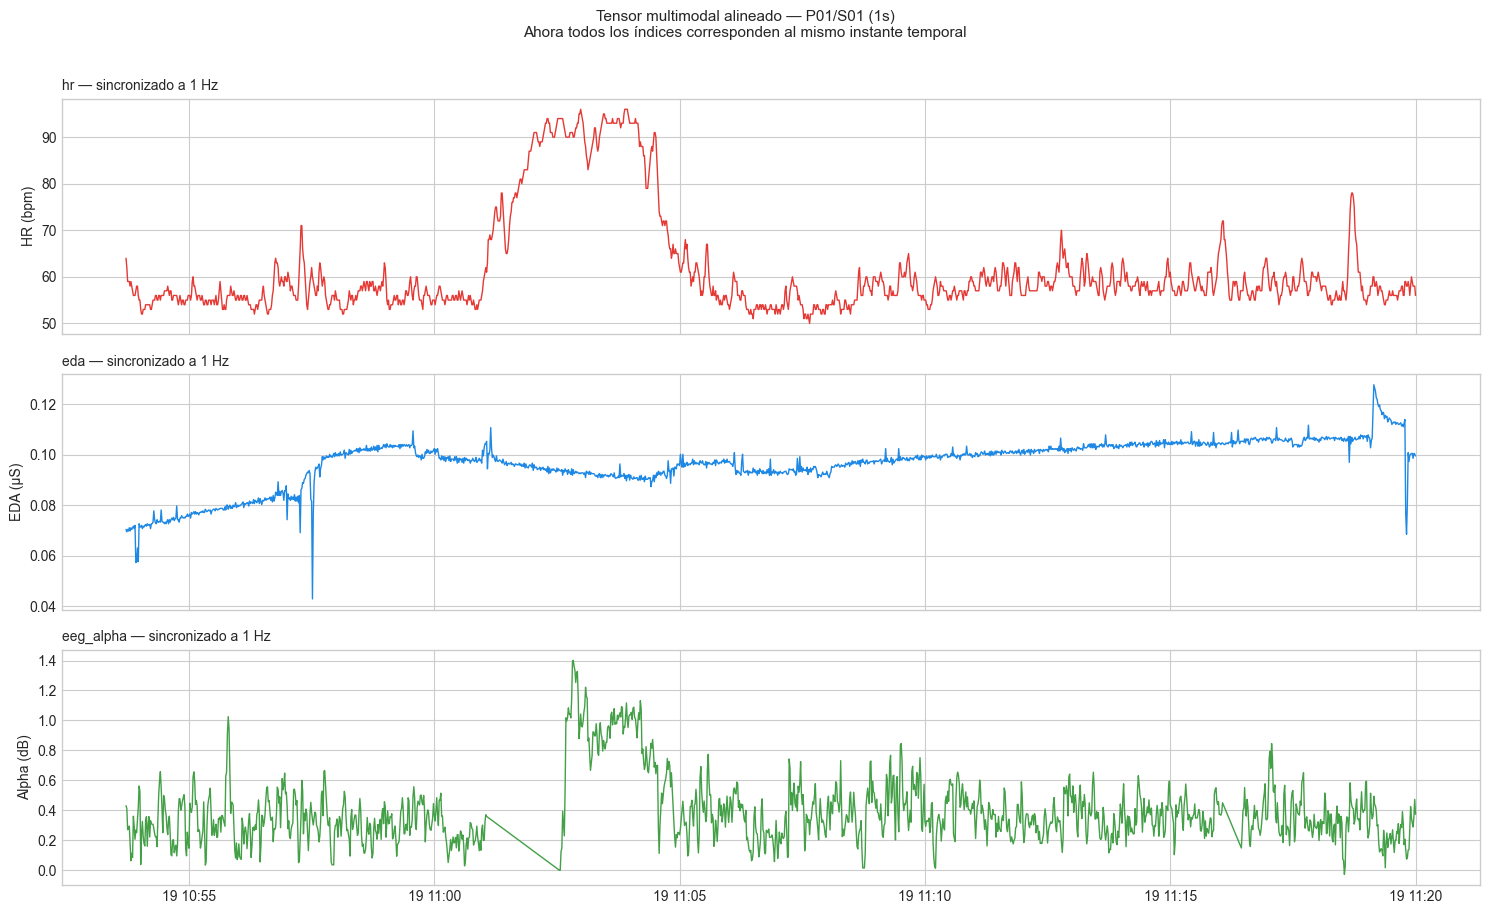
\includegraphics[width=0.88\textwidth]{figures/sincronizacion_tensor_multimodal_64hz.png}
    \caption{Pipeline completo de sincronización temporal multimodal: bioseñales de Zephyr, Empatica E4 y Muse S perfectamente alineadas y co-registradas sobre el mismo eje temporal continuo a $f_s = 64\,\text{Hz}$.}
    \label{fig:pipeline_sincronizado_multimodal}
\end{figure}

\subsection{Filtrado Digital de Bioseñales por Canal}

Para aislar las bandas fisiológicamente informativas y suprimir ruidos de movimiento e interferencias de la red eléctrica, se diseñan filtros digitales IIR tipo Butterworth bidireccionales en fase cero (\code{scipy.signal.filtfilt}):
\begin{equation}
    |H(j\omega)|^2 = \frac{1}{1 + \left( \frac{\omega}{\omega_c} \right)^{2n}}
\end{equation}
La aplicación bidireccional garantiza una respuesta de fase estrictamente nula $\phi(\omega) = 0$, evitando cualquier retardo temporal o distorsión morfológica en las ondas cardíacas o cerebrales. Los parámetros específicos por modalidad son:
\begin{itemize}
    \item \textbf{ECG (Pecho):} Pasa-banda Butterworth de 4º orden ($0.5 - 40.0\,\text{Hz}$) para eliminar derivas basales por movimiento respiratorio ($<0.5\,\text{Hz}$) y ruido electromiográfico de alta frecuencia.
    \item \textbf{EDA (Muñeca):} Pasa-bajos Butterworth de 2º orden ($f_c = 1.0\,\text{Hz}$) para suavizar la señal de conductancia cutánea previa a la extracción de respuestas galvánicas fásicas (SCR).
    \item \textbf{EEG Frontal (Muse S):} Filtro de muesca IIR (\textit{Notch}) centrado en $50\,\text{Hz}$ con factor de calidad $Q = 30$ para neutralizar el acoplamiento de la red eléctrica europea, seguido de un pasa-banda de $0.5 - 45.0\,\text{Hz}$.
    \item \textbf{BVP (Muñeca):} Pasa-banda Butterworth de 3\textsuperscript{er} orden ($0.5 - 5.0\,\text{Hz}$) adaptado al rango fisiológico de la pulsación arterial ($30 - 300\,\text{ppm}$).
\end{itemize}

El resultado cualitativo del filtrado digital en fase cero sobre las cuatro bioseñales principales se ilustra de manera comparativa en la Figura~\ref{fig:pipeline_filtrado_senales}.

\begin{figure}[htbp]
    \centering
    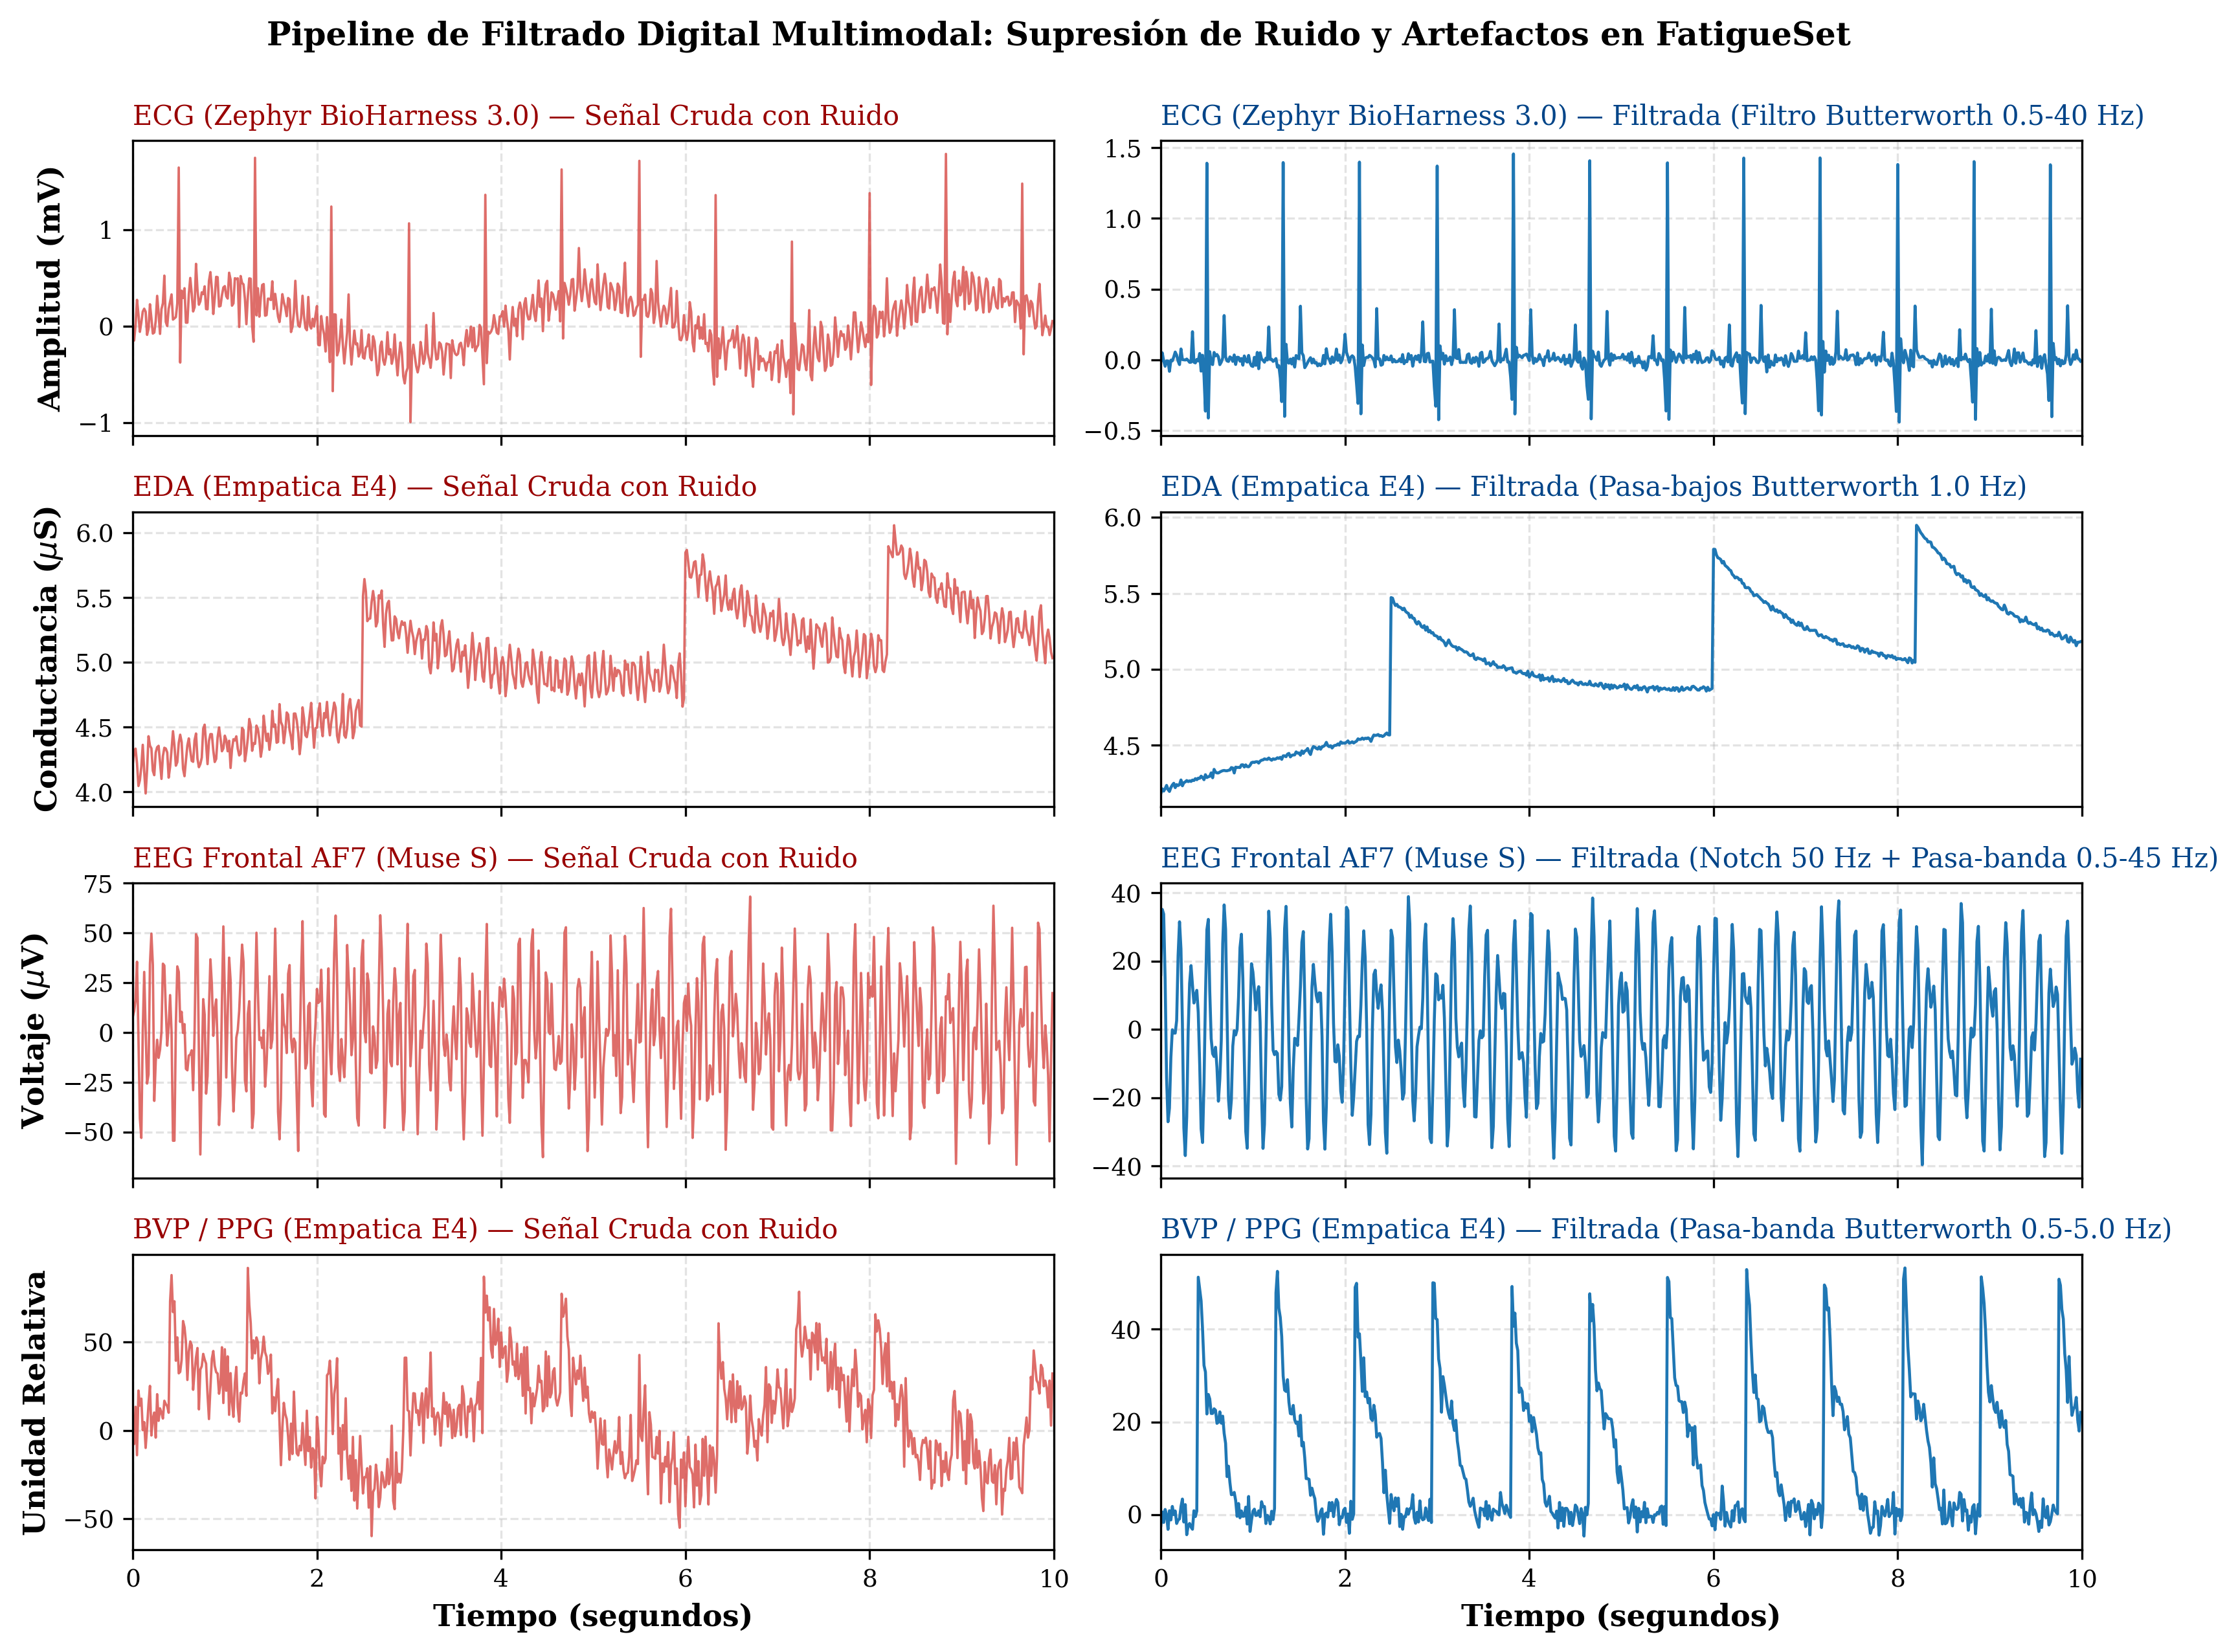
\includegraphics[width=0.88\textwidth]{figures/pipeline_filtrado_senales.png}
    \caption{Validación visual del filtrado digital multimodal: comparación de señales crudas con artefactos (columna izquierda) frente a señales limpias tras filtrado digital en fase cero (columna derecha) para ECG, EDA, EEG y BVP. (Fuente: Elaboración propia).}
    \label{fig:pipeline_filtrado_senales}
\end{figure}



\section{Segmentación en Ventanas Deslizantes y Prevención Rigurosa de Fuga de Datos}
\label{sec:windowing_leakage}

La transformación de flujos continuos de series temporales en observaciones independientes para algoritmos de Machine Learning y Deep Learning se sustenta en la técnica de ventaneo (\textit{windowing}).

\subsection{Fundamentos Teóricos de Windowing: Ventanas Deslizantes vs. Solapadas}

Una serie temporal multivariante continua $\bm{X} \in \mathbb{R}^{T \times C}$ se particiona en una colección de subsecuencias o ventanas $\mathcal{W} = \{\bm{W}_1, \bm{W}_2, \dots, \bm{W}_K\}$ de longitud fija $W$ muestras, desplazadas sucesivamente un paso de avance (\textit{step} o \textit{hop size}) $\Delta$:
\begin{equation}
    \bm{W}_k = \bm{X}[k \Delta : k \Delta + W, :], \quad k = 0, 1, \dots, K-1
\end{equation}
La relación entre $W$ y $\Delta$ define dos estrategias de partición fundamentales:
\begin{itemize}
    \item \textbf{Ventanas No Solapadas (\textit{Sliding Windows}, $\Delta = W$):} Las ventanas son contiguas sin intersección temporal. Aunque minimiza la redundancia, reduce drásticamente el número de muestras disponibles para el entrenamiento de redes profundas.
    \item \textbf{Ventanas Solapadas (\textit{Overlapping Windows}, $\Delta < W$):} Se permite un solapamiento porcentual $\text{Overlap} = \frac{W - \Delta}{W} \times 100\%$. En este proyecto se establece $W = 60\,\text{s}$ ($3840$ muestras a 64 Hz) con un desplazamiento $\Delta = 30\,\text{s}$, lo que equivale a un solapamiento exacto del $50\%$.
\end{itemize}

La Figura~\ref{fig:windowing_sliding_overlapping} ilustra visualmente cómo se extraen las primeras seis ventanas solapadas sobre la serie temporal de frecuencia cardíaca de un participante, manteniendo la continuidad contextual y duplicando el número de muestras disponibles para la optimización de los modelos neuronales.

\begin{figure}[htbp]
    \centering
    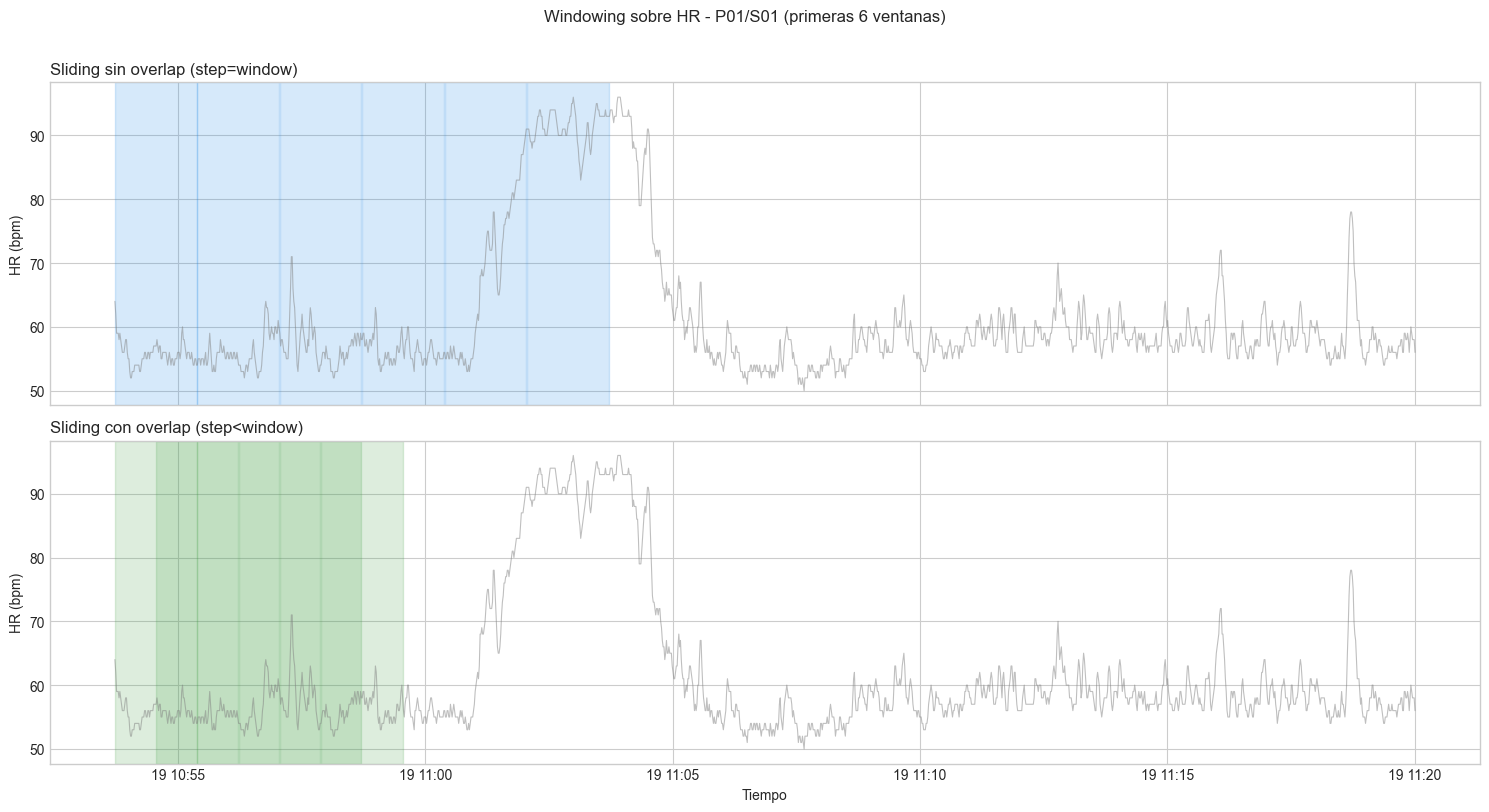
\includegraphics[width=0.88\textwidth]{figures/windowing_sliding_overlapping.png}
    \caption{Proceso didáctico de segmentación en ventanas deslizantes con solapamiento temporal del $50\%$ ($W=60\,\text{s}$, $\Delta=30\,\text{s}$) sobre la señal continua de frecuencia cardíaca (HR).}
    \label{fig:windowing_sliding_overlapping}
\end{figure}

\subsection{Análisis Crítico de las Cuatro Fugas de Datos (Data Leakage)}

La fuga de información (\textit{Data Leakage}) se define como la contaminación espuria del conjunto de entrenamiento con información que solo estaría disponible en el conjunto de prueba o en tiempo de inferencia real \cite{guillen2025libro}. En el ámbito de las bioseñales biomédicas, la fuga de datos es el principal causante de modelos con rendimientos ficticiamente perfectos en laboratorio que colapsan al ser desplegados en sujetos reales. En este TFG se han identificado y blindado cuatro modalidades críticas de fuga:

\subsubsection{Fuga 1: Partición Temporal Incorrecta y Ruptura de Causalidad}
En series temporales autorregresivas, las observaciones contiguas $x_t$ y $x_{t+1}$ exhiben una elevada autocorrelación serial $r(\tau) = \text{Corr}(x_t, x_{t+\tau})$. Si se aplica una partición aleatoria estándar (\code{train\_test\_split}), el conjunto de entrenamiento contendrá instantes futuros $t+1$ mientras que el de validación contendrá instantes pasados $t$, permitiendo al modelo "predecir el pasado basándose en el futuro". La Figura~\ref{fig:leakage_temporal_split} ilustra la diferencia entre una partición aleatoria contaminada frente a un particionado temporal cronológico estricto (\textit{Time-based Split}).

\begin{figure}[htbp]
    \centering
    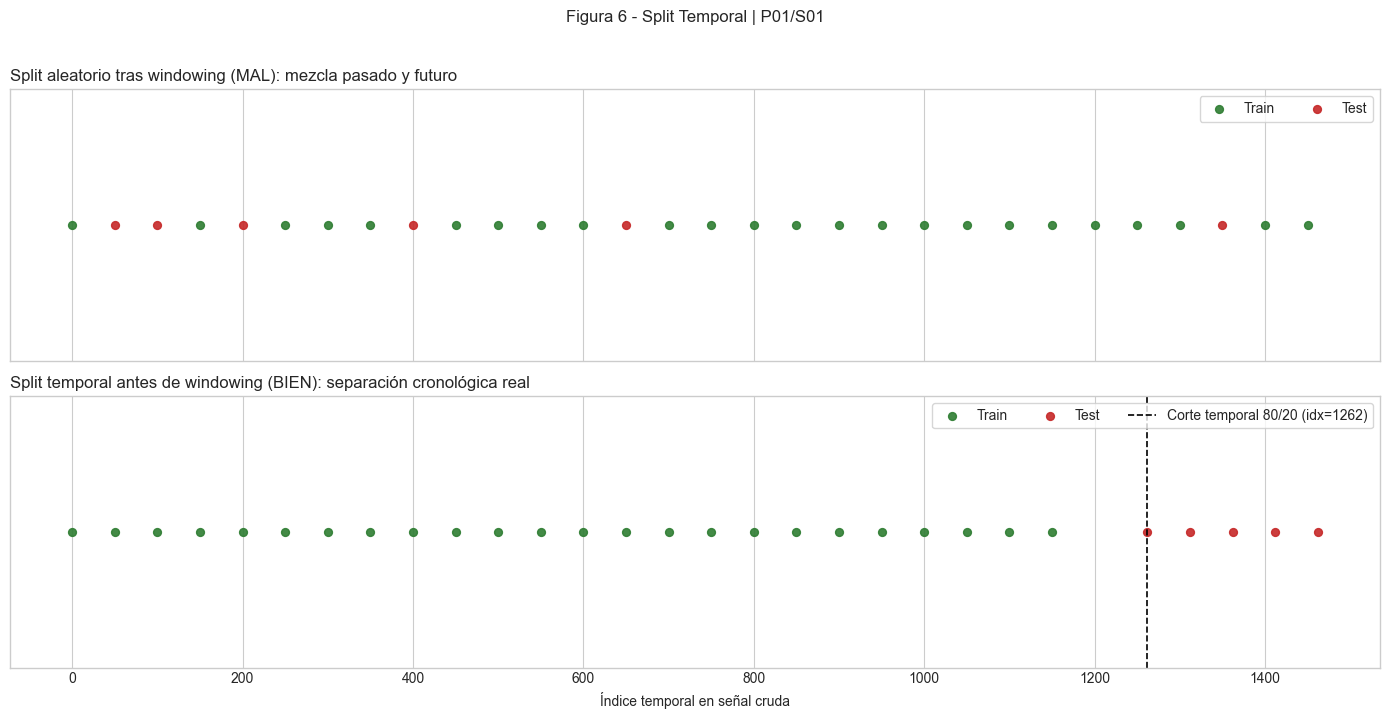
\includegraphics[width=0.88\textwidth]{figures/leakage_temporal_split.png}
    \caption{Comparación didáctica entre particionado temporal erróneo (fuga por mezcla aleatoria de instantes temporales) frente a un particionado temporal causal estricto.}
    \label{fig:leakage_temporal_split}
\end{figure}

\subsubsection{Fuga 2: Normalización Global Previa a la Partición}
Un error metodológico sumamente extendido consiste en calcular los estadísticos de normalización (media y desviación típica en Z-Score, o mínimo y máximo en MinMax) sobre la totalidad del dataset antes de dividir en entrenamiento y validación:
\begin{equation}
    \mu_{\text{global}} = \frac{1}{N_{\text{total}}}\sum_{i=1}^{N_{\text{total}}} x_i, \quad \sigma_{\text{global}} = \sqrt{\frac{1}{N_{\text{total}}}\sum_{i=1}^{N_{\text{total}}} (x_i - \mu_{\text{global}})^2}
\end{equation}
Al hacer esto, la media y la dispersión del conjunto de prueba se filtran al conjunto de entrenamiento. La Figura~\ref{fig:normalizacion_global_distribucion} muestra cómo el escalado global altera la distribución estadística. Para evitar esta contaminación, todos los transformadores y escaladores deben ajustarse (\code{fit}) de manera exclusiva sobre el subconjunto de entrenamiento de cada fold, utilizándose únicamente para transformar (\code{transform}) el subconjunto de validación.

\begin{figure}[htbp]
    \centering
    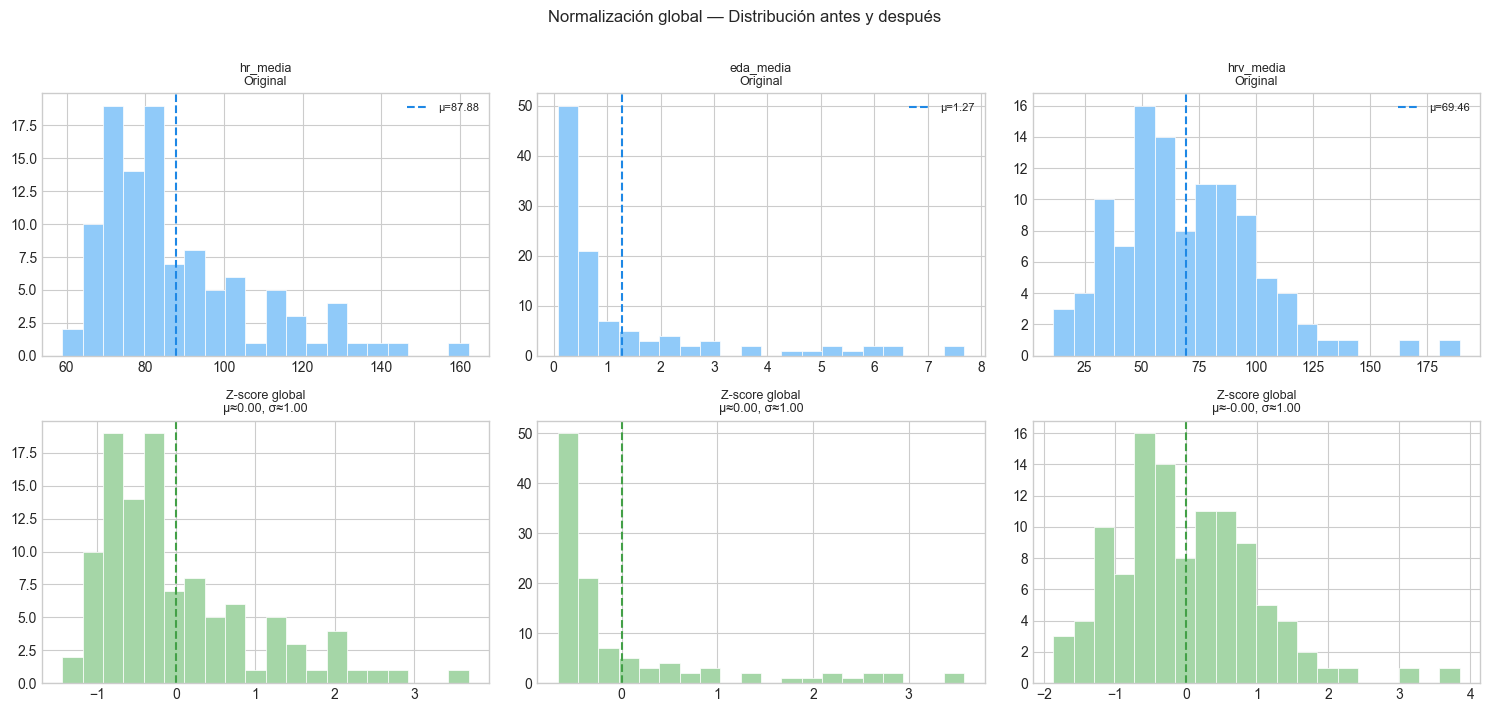
\includegraphics[width=0.88\textwidth]{figures/normalizacion_global_distribucion.png}
    \caption{Efecto de la normalización sobre la distribución estadística de bioseñales multimodales: análisis empírico de densidad y dispersión antes y después del escalado global.}
    \label{fig:normalizacion_global_distribucion}
\end{figure}

\subsubsection{Fuga 3: Solapamiento Temporal (Overlapping) en Particionado Aleatorio}
Cuando se emplea un solapamiento del $50\%$ entre ventanas consecutivas ($W_1 [0-60\,\text{s}]$ y $W_2 [30-90\,\text{s}]$), ambas ventanas comparten exactamente 30 segundos (1920 muestras a 64 Hz) de información idéntica. Si una partición aleatoria asigna $W_1$ a entrenamiento y $W_2$ a prueba, el modelo simplemente memoriza las 1920 muestras idénticas, arrojando coeficientes de determinación artificiales ($R^2 > 0.98$) que no miden generalización sino memorización.

\subsubsection{Fuga 4: Fuga de Identidad Inter-Sujeto y Protocolo GroupKFold}
Las señales biológicas de cada persona poseen una "firma biométrica" singular condicionada por su edad, sexo, capacidad aeróbica basal y anatomía electrodérmica. La Figura~\ref{fig:comparacion_normalizacion_sujeto} evidencia cómo la señal de frecuencia cardíaca de distintos participantes difiere sustancialmente en su nivel basal y rango dinámico. Si ventanas del mismo participante residen a la vez en entrenamiento y prueba, el modelo aprende a clasificar o predecir basándose en la identidad del sujeto en lugar de en los biomarcadores de fatiga.

\begin{figure}[htbp]
    \centering
    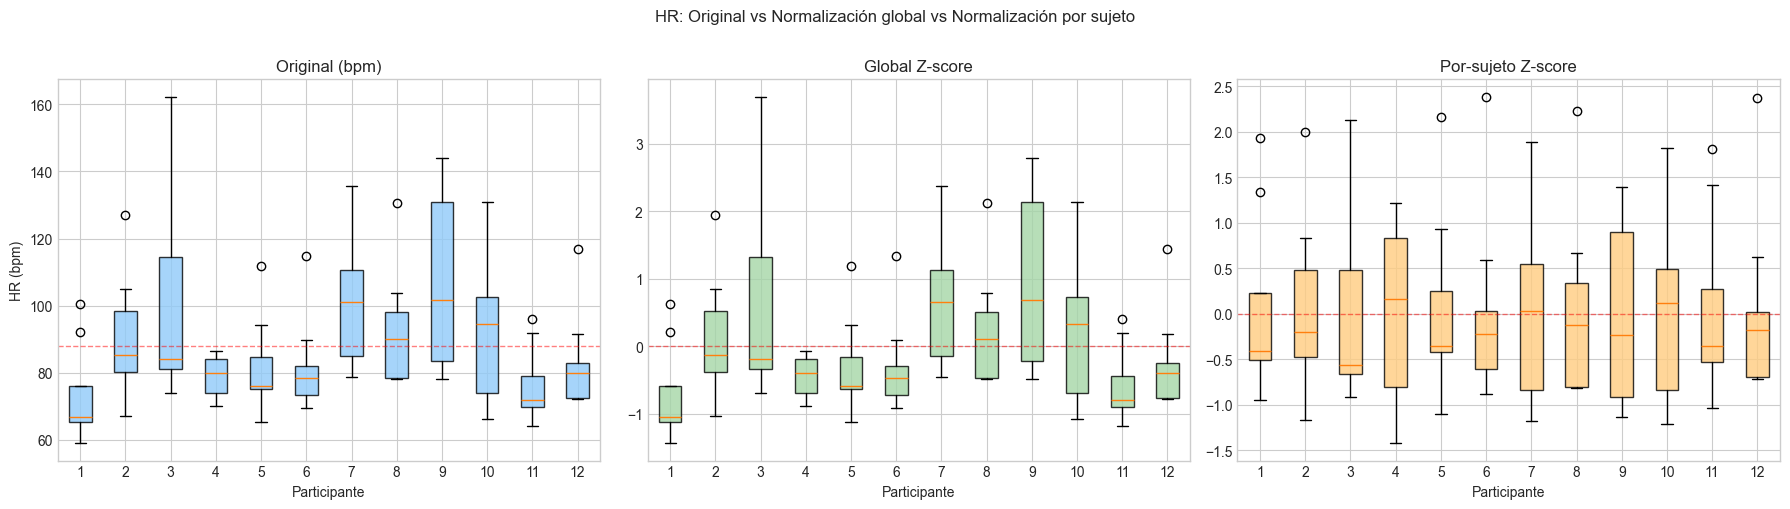
\includegraphics[width=0.88\textwidth]{figures/normalizacion_comparativa_sujeto_hr.png}
    \caption{Comparación de la señal de frecuencia cardíaca (HR) inter-sujeto: señal original frente a normalización global y adaptativa por participante, ilustrando la variabilidad biológica que justifica el uso de GroupKFold.}
    \label{fig:comparacion_normalizacion_sujeto}
\end{figure}

Para neutralizar de forma definitiva las cuatro fugas de datos, se implementa una validación cruzada estratificada por participante (\textit{GroupKFold}, $K=5$, o Leave-One-Subject-Out LOSO). Como se ilustra en el esquema de la Figura~\ref{fig:groupkfold_scheme}, la totalidad de las ventanas correspondientes a un participante específico reside de forma indivisible en el conjunto de entrenamiento o en el conjunto de prueba, evaluando siempre la capacidad de generalización ante individuos nunca vistos.

\begin{figure}[htbp]
    \centering
    \begin{tikzpicture}[node distance=0.8cm, auto,
        subj/.style={rectangle, draw=darkblue, fill=blue!10, rounded corners=5pt, text width=3.8cm, text centered, minimum height=1.0cm, font=\small\bfseries},
        win/.style={rectangle, draw=etsiitblue, fill=blue!5, rounded corners=3pt, text width=1.6cm, text centered, minimum height=0.7cm, font=\scriptsize},
        winover/.style={rectangle, draw=ugrred, fill=red!6, rounded corners=3pt, text width=1.6cm, text centered, minimum height=0.7cm, font=\scriptsize},
        line/.style={draw=darkblue, -latex', thick}]
        
        \node [subj] (p1) {Sujeto P01 (Fold 1)};
        \node [subj, right=0.6cm of p1] (p2) {Sujeto P02 (Fold 1)};
        \node [subj, right=0.6cm of p2] (p3) {Sujeto P03 (Fold 2)};
        
        \node [win, below=0.4cm of p1.south west, anchor=north west] (w1) {$W_1 [0-60\text{s}]$};
        \node [winover, below=0.4cm of p1.south east, anchor=north east] (w2) {$W_2 [30-90\text{s}]$};
        \node [win, below=0.4cm of p2] (w3) {Ventanas P02};
        \node [win, below=0.4cm of p3] (w4) {Ventanas P03};
        
        \node [above=0.15cm of p1, font=\scriptsize\bfseries, color=darkblue] {CONJUNTO DE TRAIN};
        \node [above=0.15cm of p2, font=\scriptsize\bfseries, color=darkblue] {CONJUNTO DE TRAIN};
        \node [above=0.15cm of p3, font=\scriptsize\bfseries, color=ugrred] {CONJUNTO DE TEST};
    \end{tikzpicture}
    \caption{Esquema de particionado por sujeto mediante validación cruzada estratificada \textit{GroupKFold}: todas las ventanas de un mismo participante residen exclusivamente en entrenamiento o en test, impidiendo la fuga de información.}
    \label{fig:groupkfold_scheme}
\end{figure}

\subsection{Checklist Anti-Leakage para Biometría Multimodal}

Como aportación didáctica y metodológica, se define el siguiente protocolo de verificación obligatoria aplicado en todo el proyecto:
\begin{enumerate}
    \item[$\checkmark$] \textbf{Agrupación por Sujeto:} El particionado de datos se efectúa siempre sobre identificadores únicos de participante (\code{subject\_id}), nunca sobre índices de muestra o ventanas temporales.
    \item[$\checkmark$] \textbf{Aislamiento de Escaladores:} Los objetos \code{RobustScaler} se ajustan exclusivamente sobre los pliegues de entrenamiento de cada iteración de validación cruzada.
    \item[$\checkmark$] \textbf{Orden Temporal Interno:} Dentro de cada sujeto, las ventanas preservan estrictamente su secuencia cronológica original.
    \item[$\checkmark$] \textbf{Imputación Local:} Los valores ausentes o perdidos se imputan exclusivamente con información de la ventana local actual ($<500\,\text{ms}$), sin utilizar estadísticos poblacionales futuros.
\end{enumerate}



\section{Ingeniería de Características Matemáticas y Fisiológicas}
\label{sec:feature_engineering}

Para cada ventana temporal $\mathcal{W}_k$, se extrae un vector de descriptores multidimensional $\bm{\phi}(\mathcal{W}_k) \in \mathbb{R}^D$ estructurado en tres dominios matemáticos:

\subsection{Dominio Temporal y Estadístico}
Dada una serie temporal discreta $x[n]$ con $L$ muestras ($n = 1, \dots, L$):
\begin{align}
    \text{Media: } \mu &= \frac{1}{L}\sum_{n=1}^L x[n], \quad \text{Varianza: } \sigma^2 = \frac{1}{L-1}\sum_{n=1}^L (x[n] - \mu)^2 \\
    \text{Asimetría (\textit{Skewness}): } \gamma_1 &= \frac{\frac{1}{L}\sum_{n=1}^L (x[n] - \mu)^3}{\sigma^3} \\
    \text{Curtosis (\textit{Kurtosis}): } \gamma_2 &= \frac{\frac{1}{L}\sum_{n=1}^L (x[n] - \mu)^4}{\sigma^4} - 3 \\
    \text{Valor RMS: } \text{RMS} &= \sqrt{\frac{1}{L}\sum_{n=1}^L x[n]^2}, \quad \text{Amplitud Pico a Pico: } \text{PtP} = \max(x) - \min(x)
\end{align}

\subsection{Dominio Frecuencial y Densidad Espectral de Potencia (Welch)}

La estimación de la Densidad Espectral de Potencia (PSD) $\hat{S}_{xx}(f)$ y el análisis de representaciones tiempo-frecuencia se efectúa mediante el método de Welch dividiendo la ventana de $60\,\text{s}$ en $M$ segmentos solapados con ventana Hanning $w[n]$ \cite{oppenheim1999discrete, mallat2008wavelet}:
\begin{equation}
    \hat{S}_{xx}(f) = \frac{1}{M L_s U} \sum_{m=1}^M \left| \sum_{n=0}^{L_s-1} x_m[n] w[n] e^{-j 2\pi f n / f_s} \right|^2, \quad U = \frac{1}{L_s}\sum_{n=0}^{L_s-1} w[n]^2
\end{equation}

A partir de $\hat{S}_{xx}(f)$, se integran numéricamente las potencias de banda:
\begin{itemize}
    \item \textbf{Bandas de HRV:} Muy Baja Frecuencia ($\text{VLF} < 0.04\,\text{Hz}$), Baja Frecuencia ($\text{LF}: 0.04 - 0.15\,\text{Hz}$, modulación simpática y barorrefleja), Alta Frecuencia ($\text{HF}: 0.15 - 0.40\,\text{Hz}$, tono vagal/parasimpático) y el ratio autonómico $\text{LF/HF}$.
    \item \textbf{Bandas de EEG Frontal:} Delta ($\delta: 0.5 - 4\,\text{Hz}$, sueño profundo y somnolencia), Theta ($\theta: 4 - 8\,\text{Hz}$, carga cognitiva), Alfa ($\alpha: 8 - 12\,\text{Hz}$, relajación y desactivación), Beta ($\beta: 12 - 30\,\text{Hz}$, alerta ejecutiva) y Gamma ($\gamma > 30\,\text{Hz}$). Se calculan además índices de fatiga como el ratio $\theta/\beta$ y $(\theta + \alpha) / (\alpha + \beta)$.
\end{itemize}

La Figura~\ref{fig:psd_welch_espectro} muestra la descomposición espectral estimada mediante el método de Welch para las series de HRV y EEG frontal.

\begin{figure}[htbp]
    \centering
    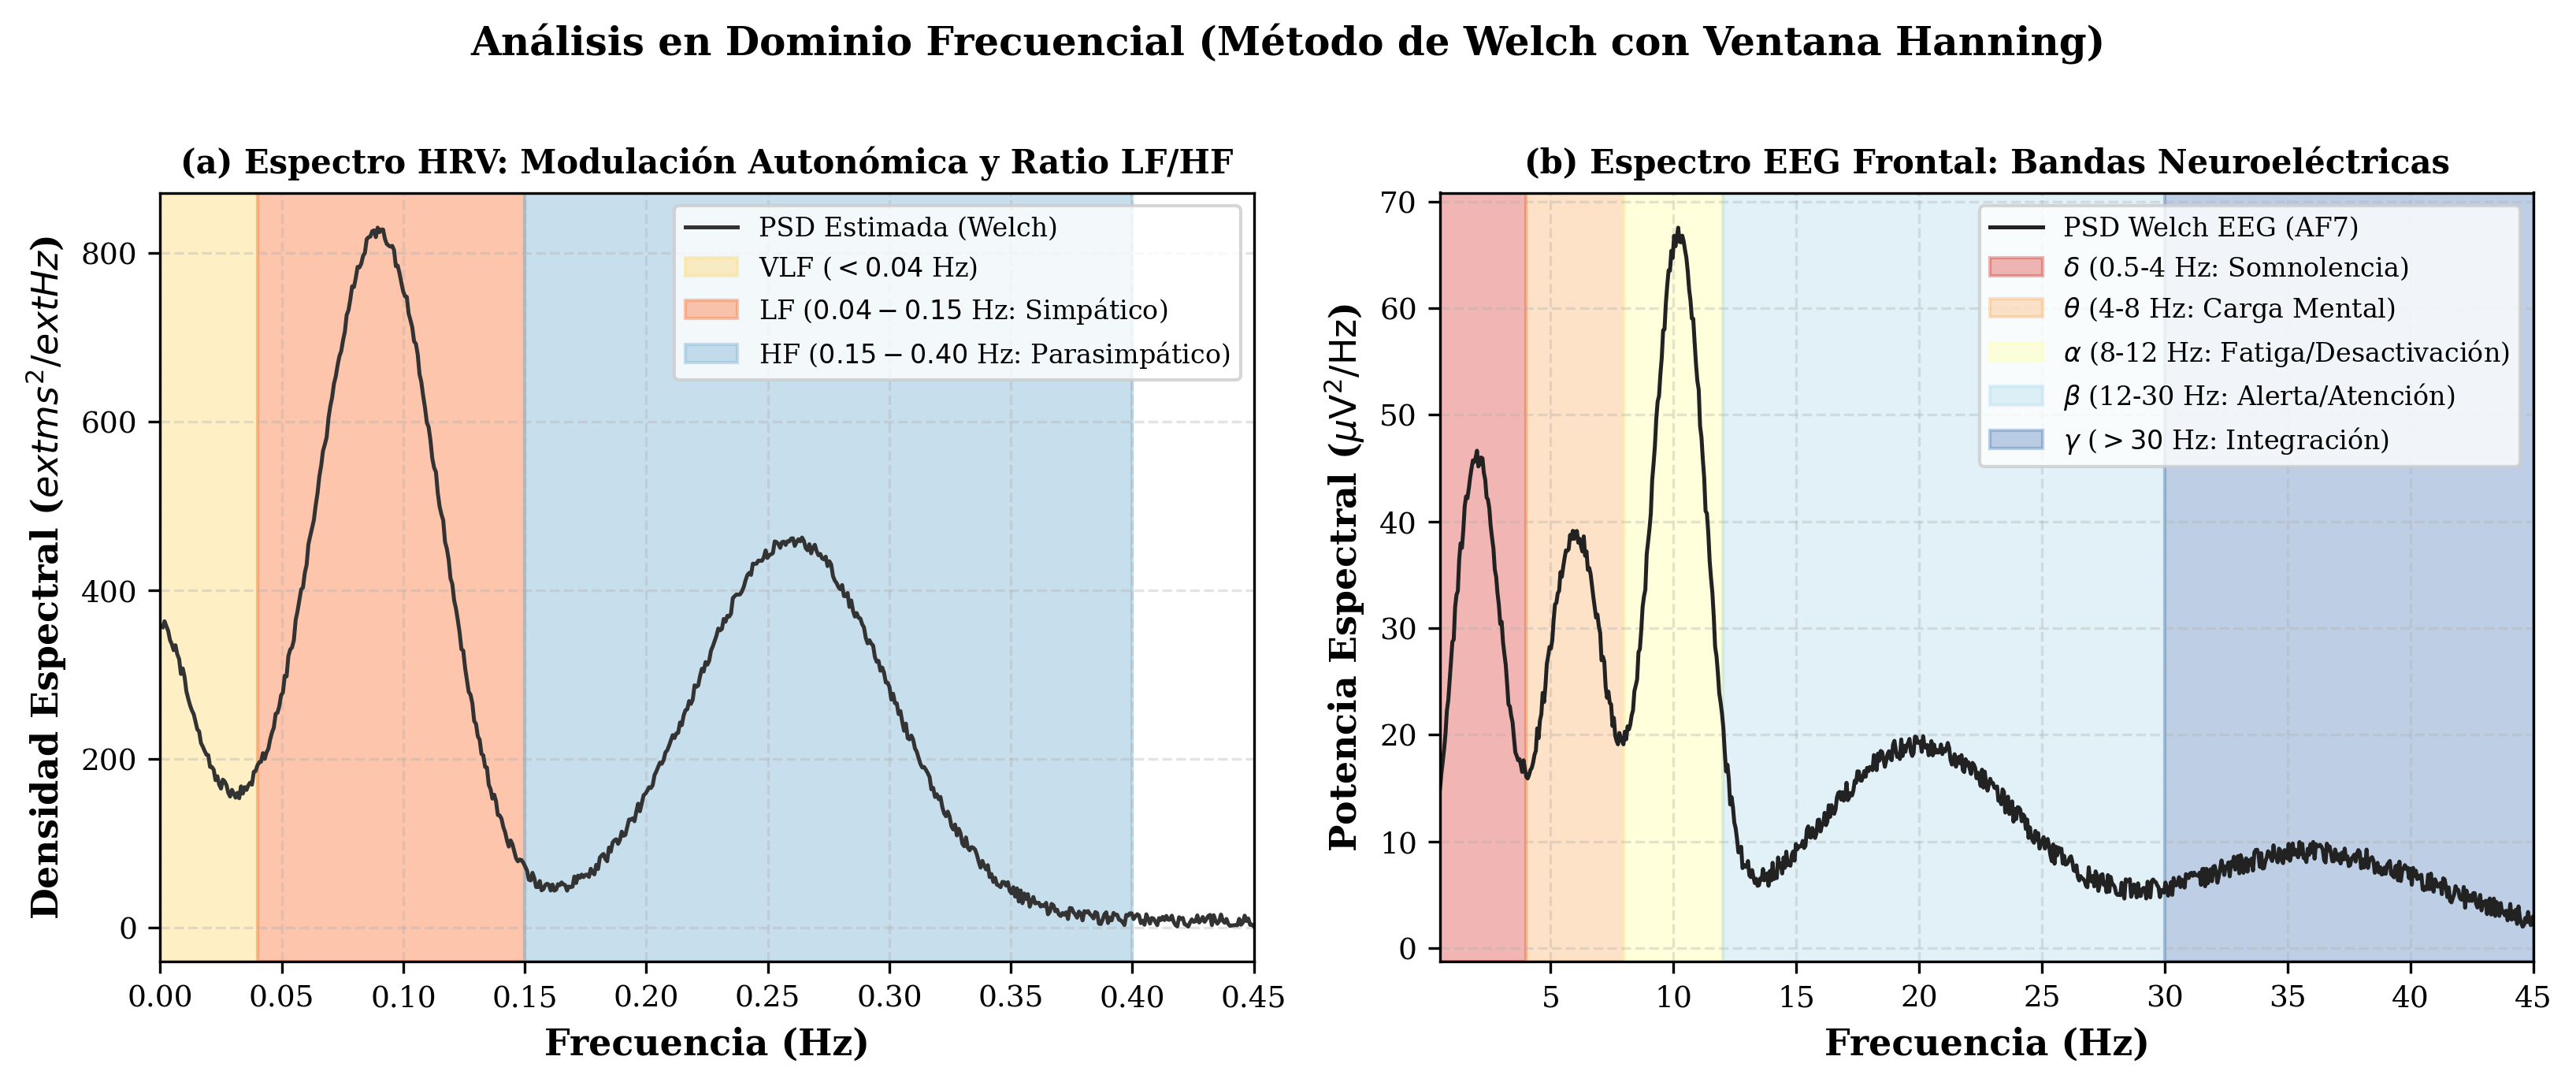
\includegraphics[width=0.92\textwidth]{figures/psd_welch_espectro.png}
    \caption{Descomposición espectral de bioseñales mediante el método de Welch: (a) Densidad espectral de HRV con segmentación en bandas VLF, LF y HF; (b) Potencia espectral de EEG frontal en electrodo AF7 con descomposición en bandas neuroeléctricas $\delta, \theta, \alpha, \beta, \gamma$. (Fuente: Elaboración propia).}
    \label{fig:psd_welch_espectro}
\end{figure}

\subsection{Dominio No Lineal y Dinámica Compleja}
\begin{itemize}
    \item \textbf{Entropía Muestral (\textit{Sample Entropy}, $\text{SampEn}$):} Cuantifica la regularidad e impredecibilidad temporal de la serie biológica:
    \begin{equation}
        \text{SampEn}(m, r, L) = -\ln \left( \frac{A^m(r)}{B^m(r)} \right)
    \end{equation}
    donde $B^m(r)$ es la probabilidad de coincidencia de patrones de longitud $m=2$ bajo un radio de tolerancia $r = 0.2 \cdot \sigma$, y $A^m(r)$ para longitud $m+1$.
    \item \textbf{Análisis de Poincaré (HRV):} Descriptores geométricos de la elipse de dispersión de intervalos $RR_i$ vs $RR_{i+1}$:
    \begin{equation}
        SD_1 = \frac{\text{RMSSD}}{\sqrt{2}}, \qquad SD_2 = \sqrt{2\,\text{SDNN}^2 - \frac{1}{2}\text{RMSSD}^2}, \qquad \text{Ratio} = \frac{SD_1}{SD_2}
    \end{equation}
\end{itemize}

\subsection{Normalización de Características}
Para evitar que canales con escalas de medida absolutas divergentes desestabilicen la optimización por gradiente en PyTorch, se aplica una normalización robusta (\textit{RobustScaler}) basada en la mediana y el rango intercuartílico:
\begin{equation}
    \tilde{x} = \frac{x - \text{mediana}(x)}{Q_{75}(x) - Q_{25}(x)}
\end{equation}
la cual exhibe una resistencia matemática superior frente a valores atípicos y artefactos mecánicos en comparación con la estandarización clásica Z-score.
